Für die Messung der Brennweite werden drei unterschiedliche Verfahren benutzt.
Für alle Messungen wird eine optische Bank verwendet, auf der die optischen Elemente in eine Richtung frei verschiebbar sind.
Als Bild wird ein L aus Perlen verwendet, welches scharf abgebildet werden soll. Für die Messungen stehen verschiedene Linsen zu Verfügung,
die eine unterschiedliche Brennweite besitzen.
\subsection{Messung der Gegenstandsweite und der Bildweite}
Auf der optischen Bank wird eine Sammellinse in einen festen Abstand $g$ vom Gegenstand platziert.
Durch das verschieben der Bildebene wird eine scharfe Abbildung gesucht. Diese befindet sich im Abstand $b$.
Nun wird $g$ variiert und das dazugehörige $b$ aufgenommen. Die Wertepaare werden in einem Graphen geplottet.
\subsection{Methode von Bessel}
Bei dieser Methode wird der Abstand zwischen Gegenstand und Bild konstant gehalten.
Durch das Verschieben der Sammellinse wird ein scharfes Bild erzeugt. Dabei gibt es zwei mögliche Stellungen für ein scharfes Bild.
Für die beiden Linsenpositionen muss gelten:
\begin{align*}
  b_1=g_2\\
  b_2=g_1
\end{align*}
Es werden die Linsenpositionen für 9 unterschiedliche Abstände $e$ besimmt.
Für $g>b$ wird das Bild verkleinert abgebildet.
Ist die Gegenstandsweite $g<b$ kleiner als die Bildweite wird das Bild vergrößert dargestellt.
In der Abblidung \ref{fig:bessel} ist der Versuchsaufbau dargestellt.
\begin{figure}[h!]
  \centering
  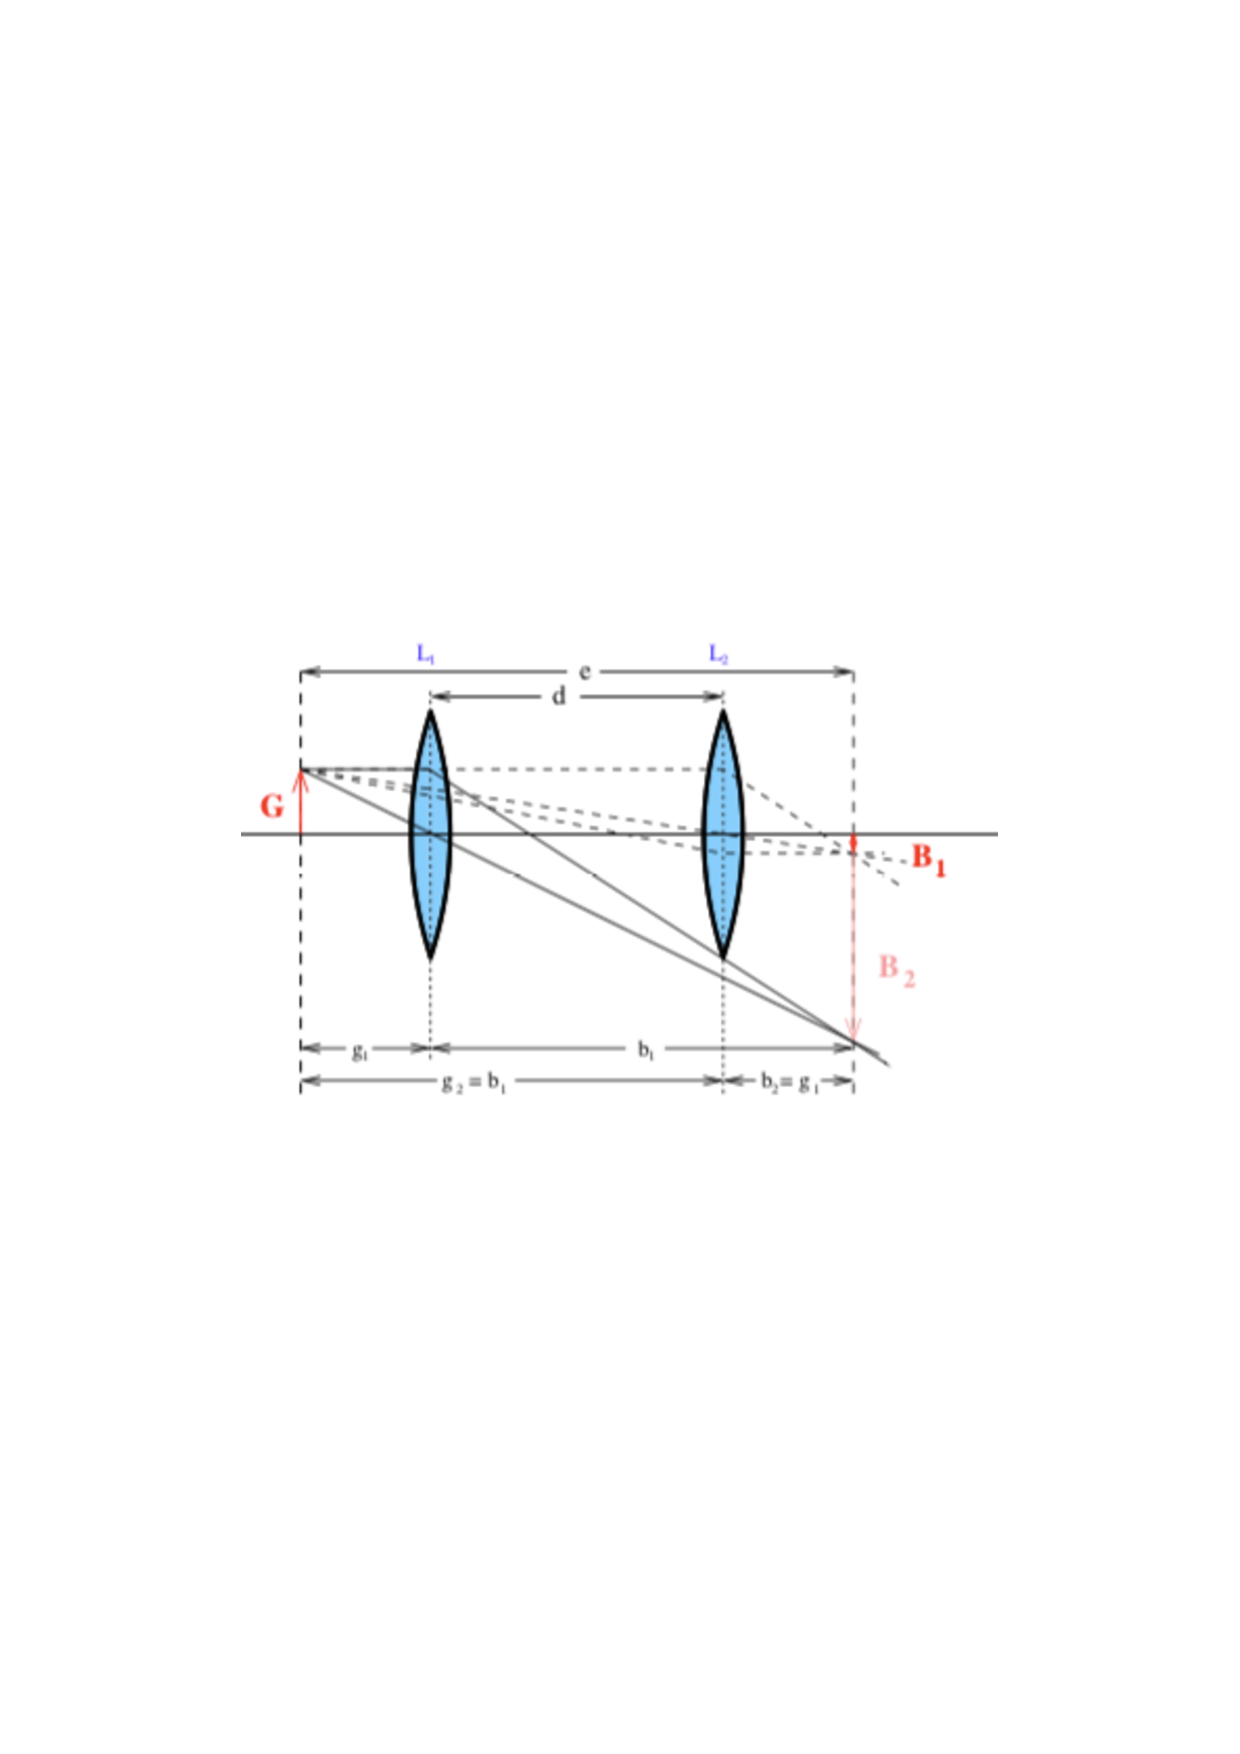
\includegraphics[width=0.7\textwidth]{theoriebessel.pdf}
  \caption{Schematischer Aufbau der Messapparatur zur Messung der Brennweite nach Bessel \cite{1}}
  \label{fig:bessel}
\end{figure}
Für den Abstand $e$ zwischen Gegenstand und Bild gilt:
\begin{align*}
  e=g_1+b_1=g_2+b_2.
\end{align*}
Der Abstand zwischen den beiden möglichen Linsenpositionen wird als $d$ bezeichnte. Für $d$ gilt:
\begin{align*}
  d=g_1-b_1=g_2-b_2
\end{align*}
Die Brennweite der Linse läst sich dann bestimmen als:
\begin{align}
  f=\frac{e^2-d^2}{4e}.
  \label{eqn:bessel}
\end{align}
Nun wird noch die chromatische Abberation mit Hilfe der Methode nach Bessel untersucht.
Dafür wir der Brennpunkt für rotes und blaues Licht bestimmt.

\subsection{Methode von Abbe}
Bei der Methode von Abbe wird die Brennweite eines Linsensystems bestimmt.
Die Mitte des Abstandes zwischen den beiden Linsen wird als A Punkt definiert.
A muss dabei nicht zwangsläufig in der Hauptebene H liegen.
Relativ zu A werden nun die Längen $g'$ und $b'$ bestimmt bei der ein scharfes Bild abbgebildet wird.
Für die beiden Abstände gilt:
\begin{align*}
  g'&=g+h=f\cdot\left(1+\frac{1}{V}\right)+h\\
  b'&=b+h'=f\cdot(1+V)+h'
\end{align*}
Durch das Messen von B und G kann über die Formel \ref{eqn:maßstab} der Abbildungsmaßstab V bestimmt werden.
Aus dem Abbildungsmaßstab V und den Länge $g'$ und $b'$ lässt sich die lage der Hauptebenen und die Brennweite $f$ bestimmen.
